%% LyX 2.1.4 created this file.  For more info, see http://www.lyx.org/.
%% Do not edit unless you really know what you are doing.
\documentclass[oneside]{amsart}
\usepackage[latin9]{inputenc}
\setlength{\parskip}{\medskipamount}
\setlength{\parindent}{0pt}
\usepackage{float}
\usepackage{mathtools}
\usepackage{amstext}
\usepackage{amsthm}
\usepackage{amssymb}
\usepackage{cancel}
\usepackage{graphicx}
\usepackage{esint}

\makeatletter
%%%%%%%%%%%%%%%%%%%%%%%%%%%%%% Textclass specific LaTeX commands.
\numberwithin{equation}{section}
\numberwithin{figure}{section}

%%%%%%%%%%%%%%%%%%%%%%%%%%%%%% User specified LaTeX commands.

%
\usepackage{amsfonts}
\usepackage{xfrac}
%\usepackage{mathabx}
\usepackage{nopageno}%%%  The following few lines affect the margin sizes. 
\usepackage{bm}
\addtolength{\topmargin}{-.5in}
\setlength{\textwidth}{6in}       
\setlength{\oddsidemargin}{.25in}              
\setlength{\evensidemargin}{.25in}         
  
\setlength{\textheight}{9in}
\renewcommand{\baselinestretch}{1}
\reversemarginpar   
%
%

\makeatother

\begin{document}

\title{ESI 6420 Homework 4 Solutions}


\author{Maksim Levental}


\date{\today}

\maketitle
Time spent: 30 hours but I don't care because this is the last homework
assignment I'll ever do in my life!

Collaborators: Chris Gianelli
\begin{enumerate}
\item [1.1]Let $q=b-Ax$ to simplify notation. Then by LP duality if $\mathcal{P}\coloneqq\min_{y}\left\{ d^{\intercal}y\big|Dy\succeq q,y\succeq0\right\} $
is infeasible for some $x\in X$ the dual $\mathcal{D}\coloneqq\max_{u}\left\{ u^{\intercal}q\big|u^{\intercal}D\preceq d^{\intercal},u\succeq0\right\} $
is unbounded. By characterization of unbounded LPs $\mathcal{D}$
being unbounded is equivalent there existing $u$ satisfying the constraints
and for which $u^{\intercal}q>0$ i.e. $u$ is an extreme ray. Therefore
$x$ is such that $\left(v^{s}\right)^{\intercal}\left(b-Ax\right)>0$
for some $s\in\left\{ 1,\dots,S\right\} $. Conversely if $\mathcal{P}$
is feasible for some $x\in X$ then, by LP duality, $\mathcal{D}$
is feasible and their optima are equal. Furthermore the optimal $u$
it's the case that $u^{\intercal}q\leq0$ and $u$ is an extreme point
and hence $\left(u^{p}\right)^{\intercal}\left(b-Ax\right)\leq0$
for some $p\in\left\{ 1,\dots,P\right\} $. Therefore both $\left(u^{p}\right)^{\intercal}\left(b-Ax\right)\leq0$
and $\left(v^{s}\right)^{\intercal}\left(b-Ax\right)\leq0$ for all
$u^{p},v^{s}$ should be the case.
\item [1.2]Let $z$ be such that $z\geq u^{\intercal}\left(b-Ax\right)=\left(u^{p}\right)^{\intercal}\left(b-Ax\right)$
since the optimum for the inner maximization is at an extreme point
of $U$. Then reformulated problem is
\begin{align*}
\min_{x,z} & \left\{ c^{\intercal}x+z\right\} \\
\text{s.t.} & \left(v^{s}\right)^{\intercal}\left(b-Ax\right)\leq0\,\forall s\\
 & \left(u^{s}\right)^{\intercal}\left(b-Ax\right)\leq z\,\forall p\\
 & x\in X
\end{align*}
or
\begin{align*}
\min_{x,z} & \left\{ c^{\intercal}x+z\right\} \\
\text{s.t.} & \left(v^{s}\right)^{\intercal}b-\left(\left(v^{s}\right)^{\intercal}A\right)x\leq0\,\forall s\\
 & \left(u^{p}\right)^{\intercal}b-\left(\left(u^{p}\right)^{\intercal}A\right)x-z\leq0\,\forall p\\
 & x\in X
\end{align*}
which is clearly linear in $x,z$.
\item [1.3]The problem is 
\begin{align*}
\min_{\mathbf{x},\mathbf{y}} & -\left(3,7\right)\cdot\mathbf{x}+\left(1,2\right)\cdot\mathbf{y}\\
\text{s.t.} & -\mathbf{1}\cdot\mathbf{x}+-\mathbf{1}\cdot\mathbf{y}\geq-4.5\\
 & -x_{1}+y_{1}\geq-1.5\\
 & -x_{2}+y_{2}\geq-.5\\
 & \mathbf{x}\in\mathbb{Z}^{+}\times\mathbb{Z}^{+}\\
 & \mathbf{y}\in\mathbb{R}^{+}\times\mathbb{R}^{+}
\end{align*}
In this instance 
\[
A=\begin{pmatrix}-1 & -1\\
-1 & 0\\
0 & -1
\end{pmatrix},D=\begin{pmatrix}-1 & -1\\
1 & 0\\
0 & 1
\end{pmatrix},b=\begin{pmatrix}-4.5\\
-1.5\\
-.5
\end{pmatrix},c=\left(-3,-7\right),d=\left(1,2\right)
\]
Then 
\begin{align*}
U & =\left\{ u\in\mathbb{R}^{3}\big|D^{\intercal}u\leq d,u\geq0\right\} \\
 & =\left\{ u\in\mathbb{R}^{3}\big|\begin{pmatrix}-1 & 1 & 0\\
-1 & 0 & 1
\end{pmatrix}\begin{pmatrix}u_{1}\\
u_{2}\\
u_{3}
\end{pmatrix}\preceq\left(1,2\right),u\geq0\right\} 
\end{align*}
 the polyhedron appears in figure \ref{fig:Bender-Polyhedron}. 
\begin{figure}[H]
\noindent \begin{centering}
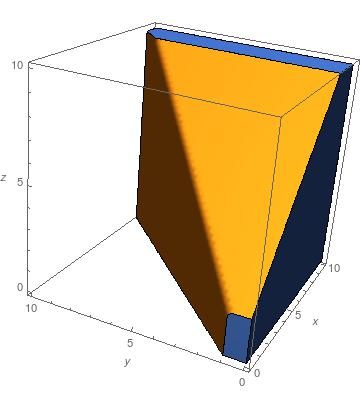
\includegraphics[scale=0.5]{Untitled-1.jpeg}\caption{Bender Polyhedron\label{fig:Bender-Polyhedron}}

\par\end{centering}

\end{figure}
Clearly the vertices are 
\begin{align*}
u^{1} & =\left(0,0,0\right)\\
u^{2} & =\left(0,1,0\right)\\
u^{3} & =\left(0,0,2\right)\\
u^{4} & =\left(0,1,2\right)
\end{align*}
and the extreme directions 
\begin{align*}
v^{1} & =\left(1,1,0\right)\\
v^{2} & =\left(1,0,1\right)\\
v^{3} & =\left(0,1,1\right)\\
v^{4} & =\left(0,0,0\right)
\end{align*}
. Therefore the Bender reformulation is 
\begin{align*}
\min_{\mathbf{x},z} & -\left(3,7\right)\cdot\mathbf{x}+z\\
\text{s.t.} & \left(0,0,0\right)\cdot\begin{pmatrix}-4.5\\
-1.5\\
-.5
\end{pmatrix}-\left(0,0,0\right)\cdot\begin{pmatrix}-1 & -1\\
-1 & 0\\
0 & -1
\end{pmatrix}\mathbf{x}\leq0\\
 & \left(0,1,0\right)\cdot\begin{pmatrix}-4.5\\
-1.5\\
-.5
\end{pmatrix}-\left(0,1,0\right)\cdot\begin{pmatrix}-1 & -1\\
-1 & 0\\
0 & -1
\end{pmatrix}\mathbf{x}\leq0\\
 & \left(0,0,2\right)\cdot\begin{pmatrix}-4.5\\
-1.5\\
-.5
\end{pmatrix}-\left(0,0,2\right)\cdot\begin{pmatrix}-1 & -1\\
-1 & 0\\
0 & -1
\end{pmatrix}\mathbf{x}\leq0\\
 & \left(0,1,2\right)\cdot\begin{pmatrix}-4.5\\
-1.5\\
-.5
\end{pmatrix}-\left(0,1,2\right)\cdot\begin{pmatrix}-1 & -1\\
-1 & 0\\
0 & -1
\end{pmatrix}\mathbf{x}\leq0\\
 & \left(1,1,0\right)\cdot\begin{pmatrix}-4.5\\
-1.5\\
-.5
\end{pmatrix}-\left(1,1,0\right)\cdot\begin{pmatrix}-1 & -1\\
-1 & 0\\
0 & -1
\end{pmatrix}\mathbf{x}-z\leq0\\
 & \left(1,0,1\right)\cdot\begin{pmatrix}-4.5\\
-1.5\\
-.5
\end{pmatrix}-\left(1,0,1\right)\cdot\begin{pmatrix}-1 & -1\\
-1 & 0\\
0 & -1
\end{pmatrix}\mathbf{x}-z\leq0\\
 & \left(0,1,1\right)\cdot\begin{pmatrix}-4.5\\
-1.5\\
-.5
\end{pmatrix}-\left(0,1,1\right)\cdot\begin{pmatrix}-1 & -1\\
-1 & 0\\
0 & -1
\end{pmatrix}\mathbf{x}-z\leq0\\
 & \left(1,0,0\right)\cdot\begin{pmatrix}-4.5\\
-1.5\\
-.5
\end{pmatrix}-\left(1,0,0\right)\cdot\begin{pmatrix}-1 & -1\\
-1 & 0\\
0 & -1
\end{pmatrix}\mathbf{x}-z\leq0\\
 & \mathbf{x}\in\mathbb{Z}^{+}\times\mathbb{Z}^{+}
\end{align*}

\item [2.1]Claim: for a continuous $f\,:\,\mathbb{R}\rightarrow\mathbb{R}$
and $h>0$ 
\[
f_{h}\left(x\right)\coloneqq\frac{1}{2h}\int_{x-h}^{x+h}f\left(t\right)dt\geq f\left(x\right)
\]
iff $f$ is convex.

\begin{proof}
$\Leftarrow$ Suppose $f$ is convex. Proceed by contradiction: suppose
there exist $h_{0},x_{0}$ such that $f\left(x_{0}\right)>f_{h_{0}}\left(x_{0}\right)$.
Since $f$ is convex there exists $g\left(x\right)=f\left(x_{0}\right)+m\left(x-x_{0}\right)$
such that $g\leq f$. But then 
\[
f\left(x_{0}\right)=\frac{1}{2h}\int_{x_{0}-h_{0}}^{x_{0}+h_{0}}g\left(t\right)dt\leq\frac{1}{2h}\int_{x_{0}-h_{0}}^{x_{0}+h_{0}}f\left(t\right)dt=f_{h_{0}}\left(x_{0}\right)
\]
a contradiction. 

$\Rightarrow$ Suppose $f_{h}\left(x\right)\geq f\left(x\right)$
for all $h,x$. Towards a contradiction suppose $f$ is not convex.
Then there exist $\lambda_{0},x_{1},x_{2}$ such that 
\[
f\left(\lambda_{0}x_{1}+\left(1-\lambda_{0}\right)x_{2}\right)>\lambda_{0}f\left(x_{1}\right)+\left(1-\lambda_{0}\right)f\left(x_{2}\right)
\]
where $\lambda_{0}\in\left(0,1\right)$. Consider the function 
\[
F\left(\lambda\right)=f\left(\lambda x_{1}+\left(1-\lambda\right)x_{2}\right)-\left(\lambda f\left(x_{1}\right)+\left(1-\lambda\right)f\left(x_{2}\right)\right)
\]
on $\left[0,1\right]$. Note that $F\left(0\right)=F\left(1\right)=0$
and $F\left(\lambda_{0}\right)>0$. Since $F$ is continuous, being
a linear function of $f$, it must achieve a maximum $F\left(\lambda^{*}\right)$
on $\left[0,1\right]$ (by the extreme value theorem) and $F\left(\lambda^{*}\right)>0$
(since $F\left(\lambda_{0}\right)>0$). Therefore there exists an
$h$-ball around $\lambda^{*}$ such that for $\lambda\in\left[\lambda^{*}-h,\lambda^{*}+h\right]$
it's the case that $F\left(\lambda\right)>0$ and without loss of
generality \footnote{Why? If $F$ is in fact constant on $\left[\lambda^{*}-h,\lambda^{*}+h\right]$
then we can take the minimum $h'>h$ such that either $\lambda^{*}-h'=0$
or $\lambda^{*}+h'=1$ and $F$ cannot be constant on $\left[\lambda^{*}-h',\lambda^{*}+h'\right]$.
This is since, depending on whether $h'$ is such that $\lambda^{*}-h'=0$
or $\lambda^{*}+h'=1$, either $F\left(\lambda^{*}-h'\right)=F\left(0\right)=0$
or $F\left(\lambda^{*}+h'\right)=F\left(1\right)=0$ (and $F$ cannot
equal zero on all $\left[\lambda^{*}-h,\lambda^{*}+h\right]$ since
$F\left(\lambda_{0}\right)>0$ and $F$ is continuous).}we can assume $F$ is not constant on $\left[\lambda^{*}-h,\lambda^{*}+h\right]$.
Then since $F\left(\lambda^{*}\right)\geq F\left(\lambda\right)$
for all $\lambda\in\left[\lambda^{*}-h,\lambda^{*}+h\right]$ and
$F\left(\lambda^{*}\right)>F\left(\lambda\right)$ for at least one
$\lambda\in\left[\lambda^{*}-h,\lambda^{*}+h\right]$ (otherwise $F$
would be constant on $\left[\lambda^{*}-h,\lambda^{*}+h\right]$)
we have that 
\[
2hF\left(\lambda^{*}\right)>\int_{\lambda^{*}-h}^{\lambda^{*}+h}F\left(\lambda\right)d\lambda
\]
which is equivalent to 
\begin{align*}
f\left(\lambda^{*}x_{1}+\left(1-\lambda^{*}\right)x_{2}\right)-\\
\left(\lambda^{*}f\left(x_{1}\right)+\left(1-\lambda^{*}\right)f\left(x_{2}\right)\right) & >\frac{1}{2h}\int_{\lambda^{*}-h}^{\lambda^{*}+h}\left[f\left(\lambda x_{1}+\left(1-\lambda\right)x_{2}\right)-\left(\lambda f\left(x_{1}\right)+\left(1-\lambda\right)f\left(x_{2}\right)\right)\right]d\lambda\\
 & =\frac{1}{2h'}\int_{\lambda^{*}-h}^{\lambda^{*}+h}f\left(\lambda x_{1}+\left(1-\lambda\right)x_{2}\right)d\lambda-\left(\lambda^{*}f\left(x_{1}\right)+\left(1-\lambda^{*}\right)f\left(x_{2}\right)\right)
\end{align*}
Cancelling $-\left(\lambda^{*}f\left(x_{1}\right)+\left(1-\lambda^{*}\right)f\left(x_{2}\right)\right)$
from both sides of the inequality we get that 
\begin{align*}
f\left(\lambda^{*}x_{1}+\left(1-\lambda^{*}\right)x_{2}\right) & >\frac{1}{2h}\int_{\lambda^{*}-h}^{\lambda^{*}+h}f\left(\lambda x_{1}+\left(1-\lambda\right)x_{2}\right)d\lambda=f_{h'}\left(\lambda^{*}x_{1}+\left(1-\lambda^{*}\right)x_{2}\right)
\end{align*}
contradicting that $f\left(x\right)\leq f_{h}\left(x\right)$ for
all. Hence $f$ must be convex.
\end{proof}
\item [2.2]Let $f\left(X\right)=-\log\left(\det\left(X\right)\right)$. 

\begin{enumerate}
\item Claim: For $X,D\succeq0$ and $X\succ0$ and $g\left(t\right)=f\left(X+tD\right)$
it's the case that 
\[
g\left(t\right)=-\log\left(\det\left(\sqrt{X}\left(I+t\left(\sqrt{X}\right)^{-1}D\left(\sqrt{X}\right)^{-1}\right)\sqrt{X}\right)\right)
\]


\begin{proof}
Firstly since $X\succ0$ it's the case that $X$ is full rank (all
nonzero eigenvalues) and there exists a matrix $\sqrt{X}$ such that
$\sqrt{X}\sqrt{X}=X$ and $\sqrt{X}$ is full rank\footnote{\begin{proof}
$\sqrt{X}=Q\sqrt{\Sigma}Q^{T}$ where $Q$ is the set of eigenvectors
corresponding to $X$ and $\sqrt{\Sigma}\succ0$ since $\Sigma\succ0$.\end{proof}
}. Then $\left(\sqrt{X}\right)^{-1}$ exists and hence 
\[
\sqrt{X}\left(\left(I+t\right)\left(\sqrt{X}\right)^{-1}D\left(\sqrt{X}\right)^{-1}\right)\sqrt{X}=X+tD
\]
and so $g\left(t\right)=-\log\left(\det\left(X+tD\right)\right)=f\left(X+tD\right)$.
\end{proof}
\item Claim: $f\left(X\right)$ is convex.

\begin{proof}
Using the representation of $g$ proven to be appropriate in part
(a) 
\begin{align*}
g\left(t\right) & =-\log\left(\det\left(\sqrt{X}\right)\det\left(I+t\left(\sqrt{X}\right)^{-1}D\left(\sqrt{X}\right)^{-1}\right)\det\left(\sqrt{X}\right)\right)\\
 & =-\log\left(\det\left(X\right)\right)-\log\left(\det\left(I+t\left(\sqrt{X}\right)^{-1}D\left(\sqrt{X}\right)^{-1}\right)\right)
\end{align*}
Let $Y=\left(\sqrt{X}\right)^{-1}D\left(\sqrt{X}\right)^{-1}$, which
is PSD since $D$ is PSD and $\left(\sqrt{X}\right)^{-1}$ is PD,
and then 
\begin{align*}
g\left(t\right) & =-\log\left(\det\left(X\right)\right)-\log\left(\det\left(I+tY\right)\right)\\
 & =-\log\left(\det\left(X\right)\right)-\log\left(\prod_{i=1}^{n}\left(1+t\lambda_{i}\right)\right)\\
 & =-\log\left(\det\left(X\right)\right)-\sum_{i=1}^{n}\log\left(1+t\lambda_{i}\right)
\end{align*}
So $g$ is convex in $t$ since it's the sum of a constant and convex
functions of linear transformations of $t$. Hence $f\left(X\right)$
is convex since it is convex on every line.
\end{proof}
\end{enumerate}
\item Claim: Let $c\sim\mathcal{N}\left(\mu,\Sigma\right)$. Then assuming
there exists $x$ such that $P\left(c^{\intercal}x\geq\alpha\right)\geq\frac{1}{2}$
\begin{align*}
\max_{x\in\mathbb{R}^{n}} & P\left(c^{\intercal}x\geq\alpha\right)\\
\text{s.t.} & Fx\leq g\\
 & Ax=b
\end{align*}
can be reformulated as a quadratic convex optimization problem.

\begin{proof}
Firstly since $c\sim\mathcal{N}\left(\mu,\Sigma\right)$ it's the
case that $X=c^{\intercal}x\sim\mathcal{N}\left(\mu\cdot x,x^{\intercal}\Sigma x\right)$
and hence
\[
P\left(X\geq\alpha\right)=P\left(\frac{X-\mu\cdot x}{\sqrt{x^{\intercal}\Sigma x}}\geq\frac{\alpha-\mu\cdot x}{\sqrt{x^{\intercal}\Sigma x}}\right)=P\left(Z\geq\frac{\alpha-\mu\cdot x}{\sqrt{x^{\intercal}\Sigma x}}\right)
\]
 where $Z\sim\mathcal{N}\left(0,1\right)$. So the maximization problem
is 
\[
\max_{x}\left[P\left(Z\geq\frac{\alpha-\mu\cdot x}{\sqrt{x^{\intercal}\Sigma x}}\right)\right]
\]
Clearly maximizing this objective is equivalent to minimizing $\frac{\alpha-\mu\cdot x}{\sqrt{x^{\intercal}\Sigma x}}$.
So the problem now is 
\begin{align*}
\min_{x\in\mathbb{R}^{n}} & \frac{\alpha-\mu\cdot x}{\sqrt{x^{\intercal}\Sigma x}}\\
\text{s.t.} & Fx\preceq g\\
 & Ax=b
\end{align*}
Alternatively we can maximize the reciprocal of the objective and
hence solve the problem
\begin{align*}
\max_{x\in\mathbb{R}^{n}} & \frac{\sqrt{x^{\intercal}\Sigma x}}{\alpha-\mu\cdot x}\\
\text{s.t.} & Fx\preceq g\\
 & Ax=b
\end{align*}
Alternatively (flipping the sign) 
\begin{align*}
\min_{x\in\mathbb{R}^{n}} & \frac{\sqrt{x^{\intercal}\Sigma x}}{\mu\cdot x-\alpha}\\
\text{s.t.} & Fx\preceq g\\
 & Ax=b
\end{align*}
The fact that there exists $x_{0}$ such that 
\[
P\left(c^{\intercal}x_{0}\geq\alpha\right)\geq\frac{1}{2}
\]
or 
\[
P\left(Z\geq\frac{\alpha-\mu\cdot x_{0}}{\sqrt{x_{0}^{\intercal}\Sigma x_{0}}}\right)\geq\frac{1}{2}
\]
or 
\[
\frac{\alpha-\mu\cdot x_{0}}{\sqrt{x_{0}^{\intercal}\Sigma x_{0}}}\leq0
\]
or
\[
\alpha-\mu\cdot x_{0}\leq0
\]
implies 
\[
\left\{ x\big|Fx\preceq g,Ax=b,\mu\cdot x-\alpha\geq0\right\} \neq\emptyset
\]
Hence let $t=\frac{1}{\alpha-\mu\cdot x}$and $y=xt$. Then an equivalent
problem is
\begin{align*}
\min_{y\in\mathbb{R}^{n}} & \sqrt{y^{\intercal}\Sigma y}\\
\text{s.t.} & Fy\preceq gt\\
 & Ay=bt\\
 & \mu\cdot y-\alpha t=1\\
 & t\geq0
\end{align*}
Squaring the objective we get a convex program with a quadratic constraint.
\end{proof}
\item [4.1]Let $x_{1}=\ln\left(r\right)$ and $x_{2}=\ln\left(h\right)$.
Note this transformation is a bijection since $r,h>0$ and $r\in\left(0,\infty\right)$
implies $x_{1}\in\left(-\infty,\infty\right)$ and similarly for $x_{2}$.
Further 
\begin{align*}
2\pi\left(r^{2}+rh\right) & =2\pi\left(e^{2x_{1}}+e^{x_{1}+x_{2}}\right)\\
\pi r^{2}h\geq V & \iff2x_{1}+x_{2}\geq\ln\left(\frac{V}{\pi}\right)
\end{align*}
Hence the two problems are equivalent.
\item [4.2]The new problem is a convex optimization problem because the
objective is convex (being the sum of two convex functions of linear
transformations) and the constraints are linear.
\item [4.3]Since everything is differentiable we can just use calculus:
let $f\left(x_{1},x_{2}\right)=2\pi\left(e^{2x_{1}}+e^{x_{1}+x_{2}}\right)$.
Then 
\[
\nabla f=\left(2e^{2x_{1}}+e^{x_{1}+x_{2}},e^{x_{1}+x_{2}}\right)
\]
Since this is never zero the constraint must be active (or the problem
unbounded). On the constraint boundary 
\[
g\left(x_{1}\right)=f\left(\ln\left(\frac{V}{\pi}\right)-2x_{1},x_{1}\right)=2\pi\left(e^{2x_{1}}+e^{x_{1}+\ln\left(\frac{V}{\pi}\right)-2x_{1}}\right)=2\pi\left(e^{2x_{1}}+e^{\ln\left(\frac{V}{\pi}\right)-x_{1}}\right)=2\pi\left(e^{2x_{1}}+\frac{V}{\pi}e^{-x_{1}}\right)
\]
Then 
\[
g'\left(x_{1}\right)=2\pi\left(2e^{2x_{1}}-\frac{V}{\pi}e^{-x_{1}}\right)
\]
which is zero at 
\[
e^{2x_{1}}=\frac{V}{2\pi}e^{-x_{1}}\Rightarrow2x_{1}=\ln\left(\frac{V}{2\pi}\right)-x_{1}\Rightarrow x_{1}=\frac{1}{3}\ln\left(\frac{V}{2\pi}\right)
\]
Therefore 
\[
x_{2}=\ln\left(\frac{V}{\pi}\right)-\frac{2}{3}\ln\left(\frac{V}{2\pi}\right)=\ln\left(2\right)+\ln\left(\frac{V}{2\pi}\right)-\frac{2}{3}\ln\left(\frac{V}{2\pi}\right)=\ln\left(2\right)+\frac{1}{3}\ln\left(\frac{V}{2\pi}\right)
\]
Hence
\begin{align*}
r & =e^{\frac{1}{3}\ln\left(\frac{V}{2\pi}\right)}=\left(\frac{V}{2\pi}\right)^{\frac{1}{3}}\\
h & =e^{\ln\left(2\right)+\frac{2}{3}\ln\left(\frac{V}{2\pi}\right)}=2\left(\frac{V}{2\pi}\right)^{\frac{1}{3}}
\end{align*}

\item [5.1]Claim: There exists an extreme point $\left(\bar{x},\bar{y}\right)$
that solves the bilinear program. 

\begin{proof}
\textbf{Full disclosure: }For this part I looked at Thieu's paper
here http://journals.math.ac.vn/acta/pdf/ 198002106.pdf.

The problem can be restated as 
\[
\min_{x\in X}\left(c^{\intercal}x+\min_{y\in Y}\left(\left(d^{\intercal}+x^{\intercal}H\right)y\right)\right)
\]
Note that $\left(\left(d^{\intercal}+x^{\intercal}H\right)y\right)$
is linear in $y$ over the polyhedron $Y$ hence the optimium is attained
at an extreme point. Let $V\left(Y\right)$ be the set of extreme
points $Y$. Then the problem can be restated again as 
\[
\min_{x\in X}\left(c^{\intercal}x+\min_{y\in V\left(Y\right)}\left(\left(d^{\intercal}+x^{\intercal}H\right)y\right)\right)
\]
For each $\bar{y}\in V\left(Y\right)$ the function 
\begin{align*}
g_{\bar{y}}\left(x\right) & =\left(\bar{y}H+c^{\intercal}\right)x+d^{\intercal}\bar{y}
\end{align*}
is a linear function of $x$. Hence the problem 
\[
\min_{x\in X}g\left(x\right)
\]
is the minimization of a piecewise linear function of $x$ over a
polyhedron and therefore attains its minimum at an extreme point $\bar{x}$.
Therefore $\left(\bar{x},\bar{y}\right)$ is a solution of the original
bilinear problem and both $\bar{x},\bar{y}$ are extreme points of
$X,Y$ respectively.
\end{proof}
\item [5.2]Claim: $\left(\hat{x},\hat{y}\right)$ is a local minimum iff
$\left(c^{\intercal}+\hat{y}^{\intercal}H^{\intercal}\right)\left(x-\hat{x}\right)\geq0$
and $\left(d^{\intercal}+\hat{x}^{\intercal}H\right)\left(y-\hat{y}\right)\geq0$
for $x,y\in X,Y$ and $\left(c^{\intercal}+\hat{y}^{\intercal}H^{\intercal}\right)\left(x-\hat{x}\right)+\left(d^{\intercal}+\hat{x}^{\intercal}H\right)\left(y-\hat{y}\right)>0$
when $\left(x-\hat{x}\right)^{\intercal}H\left(y-\hat{y}\right)<0$.

\begin{proof}
$\Rightarrow$ Assume $\left(\hat{x},\hat{y}\right)$ is a local minimum.
Then there exists some $\mathcal{N}_{\varepsilon}\left(\left(\hat{x},\hat{y}\right)\right)$
such that for all $\left(x,y\right)\in\mathcal{N}_{\varepsilon}\left(\left(\hat{x},\hat{y}\right)\right)$
it's the case that 
\[
c^{\intercal}x+d^{\intercal}y+x^{\intercal}Hy\geq c^{\intercal}\hat{x}+d^{\intercal}\hat{y}+\hat{x}^{\intercal}H\hat{y}
\]
$\hat{x}$ being optimal implies that for any $\left(x,\hat{y}\right)\in\mathcal{N}_{\varepsilon}\left(\left(\hat{x},\hat{y}\right)\right)$
\begin{align*}
c^{\intercal}x+d^{\intercal}\hat{y}+x^{\intercal}H\hat{y} & \geq c^{\intercal}\hat{x}+d^{\intercal}\hat{y}+\hat{x}^{\intercal}H\hat{y}\\
 & \iff\\
c^{\intercal}\left(x-\hat{x}\right)+x^{\intercal}H\hat{y} & \geq\hat{x}^{\intercal}H\hat{y}\\
 & \iff\\
c^{\intercal}\left(x-\hat{x}\right)+\left(x-\hat{x}\right)^{\intercal}H\hat{y} & \geq0
\end{align*}
Since $u^{\intercal}Av=\left(u^{\intercal}Av\right)^{\intercal}=v^{\intercal}A^{\intercal}u$
for all $u,v,A$ 
\begin{align*}
c^{\intercal}\left(x-\hat{x}\right)+\left(x-\hat{x}\right)^{\intercal}H\hat{y} & \geq0\\
 & \iff\\
c^{\intercal}\left(x-\hat{x}\right)+\hat{y}^{\intercal}H^{\intercal}\left(x-\hat{x}\right) & \geq0\\
 & \iff\\
\left(c^{\intercal}+\hat{y}^{\intercal}H^{\intercal}\right)\left(x-\hat{x}\right) & \geq0
\end{align*}
Similarly for $\left(\hat{x},y\right)\in\mathcal{N}_{\varepsilon}\left(\left(\hat{x},\hat{y}\right)\right)$
\begin{align*}
d^{\intercal}y+\hat{x}^{\intercal}Hy & \geq d^{\intercal}\hat{y}+\hat{x}^{\intercal}H\hat{y}\\
 & \iff\\
d^{\intercal}\left(y-\hat{y}\right)+\hat{x}^{\intercal}Hy-\hat{x}^{\intercal}H\hat{y} & \geq0\\
 & \iff\\
d^{\intercal}\left(y-\hat{y}\right)+\hat{x}^{\intercal}H\left(y-\hat{y}\right) & \geq0\\
 & \iff\\
\left(d^{\intercal}+\hat{x}^{\intercal}H\right)\left(y-\hat{y}\right) & \geq0
\end{align*}
Further if $\left(\hat{x},\hat{y}\right)$ is a local minimum
\begin{align*}
c^{\intercal}x+d^{\intercal}y+x^{\intercal}Hy & \geq c^{\intercal}\hat{x}+d^{\intercal}\hat{y}+\hat{x}^{\intercal}H\hat{y}\\
 & \iff\\
c^{\intercal}\left(x-\hat{x}\right)+d^{\intercal}\left(y-\hat{y}\right)+x^{\intercal}Hy-\hat{x}^{\intercal}H\hat{y} & \geq0\\
 & \iff\\
c^{\intercal}\left(x-\hat{x}\right)+d^{\intercal}\left(y-\hat{y}\right)+\left(x^{\intercal}-\hat{x}^{\intercal}\right)H\left(y-\hat{y}\right)+\left(-2\hat{x}^{\intercal}H\hat{y}+x^{\intercal}H\hat{y}+\hat{x}^{\intercal}Hy\right) & \geq0
\end{align*}
Now since $\left(x-\hat{x}\right)^{\intercal}H\left(y-\hat{y}\right)<0$
\begin{align*}
c^{\intercal}\left(x-\hat{x}\right)+d^{\intercal}\left(y-\hat{y}\right)+\left(-2\hat{x}^{\intercal}H\hat{y}+x^{\intercal}H\hat{y}+\hat{x}^{\intercal}Hy\right) & >0\\
 & \iff\\
c^{\intercal}\left(x-\hat{x}\right)+d^{\intercal}\left(y-\hat{y}\right)+\left(x^{\intercal}-\hat{x}^{\intercal}\right)H\hat{y}+\hat{x}^{\intercal}H\left(y-\hat{y}\right) & >0\\
 & \iff\\
\left(c^{\intercal}+\hat{y}^{\intercal}H^{\intercal}\right)\left(x-\hat{x}\right)+\left(d^{\intercal}+\hat{x}^{\intercal}H\right)\left(y-\hat{y}\right) & >0
\end{align*}
Finally since, by part (1), since a solution exists at an extreme
point, these inequalities hold for all $\left(x,y\right)\in X\times Y$.
\begin{proof}
$\Leftarrow$ Assume the inequalities hold for $\left(x,y\right)\in X\times Y$
and $\left(x-\hat{x}\right)^{\intercal}H\left(y-\hat{y}\right)\geq0$.
Then 
\begin{align*}
\left(c^{\intercal}+\hat{y}^{\intercal}H^{\intercal}\right)\left(x-\hat{x}\right)+\left(d^{\intercal}+\hat{x}^{\intercal}H\right)\left(y-\hat{y}\right)+\left(x-\hat{x}\right)^{\intercal}H\left(y-\hat{y}\right) & \geq0\\
 & \iff\\
c^{\intercal}\left(x-\hat{x}\right)+d^{\intercal}\left(y-\hat{y}\right)\cancel{+\hat{y}^{\intercal}H^{\intercal}x}-\hat{y}^{\intercal}H^{\intercal}\hat{x}\cancel{+\hat{x}^{\intercal}Hy}\cancel{-\hat{x}^{\intercal}H\hat{y}}+x^{\intercal}Hy\cancel{-\hat{x}^{\intercal}Hy}\cancel{-x^{\intercal}H\hat{y}}\cancel{+\hat{x}^{\intercal}H\hat{y}} & \geq0\\
 & \iff\\
c^{\intercal}\left(x-\hat{x}\right)+d^{\intercal}\left(y-\hat{y}\right)+x^{\intercal}Hy & \geq\hat{y}^{\intercal}H^{\intercal}\hat{x}\\
 & \iff\\
c^{\intercal}x+d^{\intercal}y+x^{\intercal}Hy & \geq c^{\intercal}\hat{x}+d^{\intercal}\hat{y}+\hat{y}^{\intercal}H^{\intercal}\hat{x}
\end{align*}
If for $\left(x,y\right)$ it's the case that $\left(x-\hat{x}\right)^{\intercal}H\left(y-\hat{y}\right)<0$
then 
\begin{align*}
\left(c^{\intercal}+\hat{y}^{\intercal}H^{\intercal}\right)\left(x-\hat{x}\right)+\left(d^{\intercal}+\hat{x}^{\intercal}H\right)\left(y-\hat{y}\right) & >0\\
 & \iff\\
\left(c^{\intercal}+\hat{y}^{\intercal}H^{\intercal}\right)\left(x-\hat{x}\right)+\left(d^{\intercal}+\hat{x}^{\intercal}H\right)\left(y-\hat{y}\right)+\left(x^{\intercal}-\hat{x}^{\intercal}\right)H\left(y-\hat{y}\right) & \geq0\\
 & \iff\\
c^{\intercal}x+d^{\intercal}y+x^{\intercal}Hy & \geq c^{\intercal}\hat{x}+d^{\intercal}\hat{y}+\hat{x}^{\intercal}H\hat{y}
\end{align*}

\end{proof}
\end{proof}
\item [5.3]Claim: $\left(\hat{x},\hat{y}\right)$ is a KKT point iff $\left(c^{\intercal}+\hat{y}^{\intercal}H^{\intercal}\right)\left(x-\hat{x}\right)\geq0$
and $\left(d^{\intercal}+\hat{x}^{\intercal}H\right)\left(y-\hat{y}\right)\geq0$
for $x,y\in X,Y$

\begin{proof}
Suppose $\left(\hat{x},\hat{y}\right)$ is a KKT point. By Gordan's
theorem there exists no feasible $\left(x,y\right)$ such that 
\[
\left(\left.\nabla f\left(x,y\right)\right|_{\left(x,y\right)=\left(\hat{x},\hat{y}\right)}\right)^{\intercal}\left(x-\hat{x},y-\hat{y}\right)<0
\]
where $f\left(x,y\right)=c^{\intercal}x+d^{\intercal}y+x^{\intercal}Hy$.
Therefore for feasible all $\left(x,y\right)$
\[
\left(\left.\nabla f\left(x,y\right)\right|_{\left(x,y\right)=\left(\hat{x},\hat{y}\right)}\right)^{\intercal}\left(x-\hat{x},y-\hat{y}\right)\geq0
\]
Finally note that 
\[
\left(\left.\nabla f\left(x,y\right)\right|_{\left(x,y\right)=\left(\hat{x},\hat{y}\right)}\right)^{\intercal}=\left(c^{\intercal}+\hat{y}^{\intercal}H^{\intercal},d^{\intercal}+\hat{x}^{\intercal}H\right)^{\intercal}
\]


Since Gordan's theorem is iff the proof works in both directions.
\end{proof}
\item [5.4]For $f\left(x_{1},x_{2},y_{1},y_{2}\right)=x_{2}+y_{1}+x_{2}y_{1}-x_{1}y_{2}+x_{2}y_{2}$
we have that $c=\left(0,1\right),d=\left(1,0\right)$ and 
\[
H=\begin{pmatrix}0 & -1\\
1 & 1
\end{pmatrix}
\]
The point $\left(x_{1},x_{2},y_{1},y_{2}\right)=\left(0,0,0,0\right)$
is a KKT point since 
\[
\left(c^{\intercal}+\hat{y}^{\intercal}H^{\intercal}\right)\left(x-\hat{x}\right)=\left(0,1\right)^{\intercal}x\geq0
\]
for $\left(x_{1},x_{2}\right)\in X$ (since $x_{2}\geq0$ for $x\in X$)
and
\[
\left(d^{\intercal}+\hat{x}^{\intercal}H\right)\left(y-\hat{y}\right)=\left(1,0\right)^{\intercal}y\geq0
\]
for $\left(y_{1},y_{2}\right)\in Y$ (since $y_{1}\geq0$ for $y\in Y$).
The point $\left(0,0,0,0\right)$ is not a local minimum though since
for $\left(x_{1},x_{2}\right)=\left(a,0\right)$ and $\left(y_{1},y_{2}\right)=\left(0,b\right)$
we have that 
\[
\left(x-\hat{x}\right)^{\intercal}H\left(y-\hat{y}\right)=x^{\intercal}Hy=x_{2}y_{1}-x_{1}y_{2}+x_{2}y_{2}=-ab<0
\]
and yet 
\[
x_{2}+y_{1}=0+0\not>0
\]
and hence by part (2) $\left(a,0,0,b\right)$ is not a local minimum.
On the other hand for $\left(x_{1},x_{2},y_{1},y_{2}\right)=\left(3,0,1,5\right)$
\[
\left(0,1\right)^{\intercal}\left(3,0\right)=0\geq0
\]
and
\[
\left(1,0\right)^{\intercal}\left(1,5\right)=1\geq0
\]
and
\[
\left(x-\hat{x}\right)^{\intercal}H\left(y-\hat{y}\right)=x^{\intercal}Hy=-3\times5<0
\]
and
\[
\left(0,1\right)^{\intercal}\left(3,0\right)+\left(1,0\right)^{\intercal}\left(1,5\right)=1>0
\]
The global minimum is indeed at $\left(3,0,1,5\right)$ with $f\left(3,0,1,5\right)=-14$.
\item [6.1]Let $P$ be the program 
\begin{align*}
\min_{x} & -\ln\left(a^{\intercal}x\right)-\ln\left(b^{\intercal}x\right)\\
\text{s.t.} & \mathbf{1}^{\intercal}x=1,x\succeq0
\end{align*}
which is equivalent
\begin{align*}
\min_{x} & -\ln\left(a^{\intercal}x\right)-\ln\left(b^{\intercal}x\right)\\
\text{s.t.} & \mathbf{1}^{\intercal}x-1=0,-x\preceq0
\end{align*}
Since the objective is differentiable and each of the constraints
is differentiable the KKT conditions are
\begin{align*}
-\frac{a}{a^{\intercal}x}-\frac{b}{b^{\intercal}x}+u_{0}\mathbf{1}-\left(u_{1},\dots,u_{n}\right) & =0\\
u_{0}\left(\mathbf{1}^{\intercal}x-1\right) & =0\\
-\left(u_{1}x_{1},\dots,u_{n}x_{n}\right) & =0\\
\left(u_{1},\dots,u_{n}\right) & \succeq0\\
u_{0} & \in\mathbb{R}
\end{align*}
with $\left\{ \mathbf{1}^{\intercal}x-1,-u_{1}x_{1},\dots,-u_{n}x_{n}\right\} $
linearly independent.
\item [6.2]Let $x=\left(\frac{1}{2},0,\dots,0,\frac{1}{2}\right)$. Since
the problem is convex, if a point satisfies the KKT conditions then
it's a global minimum. To wit 
\begin{align*}
-\frac{a}{a^{\intercal}x}-\frac{b}{b^{\intercal}x}+u_{0}\mathbf{1}-\left(u_{1},\dots,u_{n}\right) & =-\frac{a}{\frac{1}{2}\left(a_{1}+a_{n}\right)}-\frac{b}{\frac{1}{2}\left(\frac{1}{a_{1}}+\frac{1}{a_{n}}\right)}+u_{0}\mathbf{1}-\left(u_{1},\dots,u_{n}\right)=0\\
u_{0}\left(\mathbf{1}^{\intercal}\left(\frac{1}{2},0,\dots,0,\frac{1}{2}\right)-1\right) & =u_{0}\times0=0\\
-\left(\frac{1}{2}u_{1},0,\dots,0,\frac{1}{2}u_{n}\right) & =0
\end{align*}
Therefore $u_{1}=u_{n}=0$ and otherwise $u_{i}\neq0$. Hence for
$u_{0}=2$ and $u_{i}=2\left(1-\frac{a_{i}+\frac{a_{1}a_{n}}{a_{i}}}{a_{1}+a_{n}}\right)$
for $i=2,\dots,n-1$
\begin{align*}
-\frac{a}{\frac{1}{2}\left(a_{1}+a_{n}\right)}-\frac{b}{\frac{1}{2}\left(\frac{1}{a_{1}}+\frac{1}{a_{n}}\right)}+u_{0}\mathbf{1}-\left(0,u_{2}\dots,u_{n-1},0\right) & =\left(u_{0},u_{0}-u_{2},\dots,u_{0}-u_{n-1},u_{0}\right)-\frac{2}{\left(a_{1}+a_{n}\right)}\left(a+a_{1}a_{n}b\right)\\
 & =\left(u_{0},u_{0}-u_{2},\dots,u_{0}-u_{n-1},u_{0}\right)\\
 & -\frac{2}{\left(a_{1}+a_{n}\right)}\left(a_{1}+a_{1}a_{n}b_{1},a_{2}+a_{1}a_{n}b_{2},\dots,a_{n}+a_{1}a_{n}b_{n}\right)\\
 & =\left(u_{0},u_{0}-u_{2},\dots,u_{0}-u_{n-1},u_{0}\right)\\
 & -\frac{2}{\left(a_{1}+a_{n}\right)}\left(a_{1}+a_{n},a_{2}+a_{1}a_{n}b_{2},\dots,a_{n}+a_{1}\right)\\
 & =\left(u_{0},u_{0}-u_{2},\dots,u_{0}-u_{n-1},u_{0}\right)-2\left(1,\frac{a_{2}+\frac{a_{1}a_{n}}{a_{2}}}{a_{1}+a_{n}},\dots,1\right)\\
 & =\left(u_{0}-2,u_{0}-2\left(\frac{a_{2}+\frac{a_{1}a_{n}}{a_{2}}}{a_{1}+a_{n}}\right)-u_{2},\dots,u_{0}-2\right)\\
 & =\left(0,2\left(1-\frac{a_{2}+\frac{a_{1}a_{n}}{a_{2}}}{a_{1}+a_{n}}\right)-u_{2},\dots,0\right)\\
 & =0
\end{align*}
All that remains is to show that $u_{i}\geq0$ (since $u_{0}$ is
free). Note that 
\[
\left(a_{i}-\frac{\left(a_{1}+a_{n}\right)}{2}\right)^{2}\leq\left(a_{n}-\frac{\left(a_{1}+a_{n}\right)}{2}\right)^{2}
\]
since $a_{1}\leq a_{i}\leq a_{n}$ (i.e. any $a_{i}$ is closer to
the ``middle'' {[}average{]} than $a_{n}$). And I claim I'm done.
Why?
\[
\left(a_{i}-\frac{\left(a_{1}+a_{n}\right)}{2}\right)^{2}=a_{i}^{2}-a_{i}\left(a_{1}+a_{n}\right)+\left(\frac{\left(a_{1}+a_{n}\right)}{2}\right)^{2}
\]
and
\[
\left(a_{n}-\frac{\left(a_{1}+a_{n}\right)}{2}\right)^{2}=\left(\frac{\left(a_{1}+a_{n}\right)}{2}\right)^{2}-a_{1}a_{n}
\]
and therefore
\[
a_{i}^{2}-a_{i}\left(a_{1}+a_{n}\right)\leq-a_{1}a_{n}
\]
or
\[
a_{i}^{2}+a_{1}a_{n}\leq a_{i}\left(a_{1}+a_{n}\right)
\]
or
\[
\frac{a_{i}+\frac{a_{1}a_{n}}{a_{i}}}{a_{1}+a_{n}}\leq1
\]
Hence
\[
u_{i}=2\left(1-\frac{a_{i}+\frac{a_{1}a_{n}}{a_{i}}}{a_{1}+a_{n}}\right)\geq2\left(1-1\right)=0
\]
Finally $z^{*}=-\ln\left(\frac{a_{1}}{2}+\frac{a_{n}}{2}\right)-\ln\left(\frac{1}{2a_{1}}+\frac{1}{2a_{n}}\right)=-\ln\left(\frac{\left(a_{1}+a_{n}\right)^{2}}{4a_{1}a_{n}}\right)$.
\item [6.3]Claim: for Hermitian pd $A$ 
\[
2\sqrt{u^{\intercal}Au}\sqrt{u^{\intercal}A^{-1}u}\leq\sqrt{\frac{\lambda_{1}}{\lambda_{n}}}+\sqrt{\frac{\lambda_{n}}{\lambda_{1}}}
\]


\begin{proof}
Let $A=V\Sigma V^{\intercal}$ then $V^{\intercal}\Sigma V=A$ and
$V^{\intercal}\Sigma^{-1}V=A^{-1}$ 
\[
\sqrt{u^{\intercal}Au}\sqrt{u^{\intercal}A^{-1}u}=\sqrt{u^{\intercal}V^{\intercal}\Sigma Vu}\sqrt{u^{\intercal}V^{\intercal}\Sigma^{-1}Vu}
\]
Let $v=Vu$. Therefore 
\[
\sqrt{u^{\intercal}Au}\sqrt{u^{\intercal}A^{-1}u}=\sqrt{v^{\intercal}\Sigma v}\sqrt{v^{\intercal}\Sigma^{-1}v}
\]
Taking log of $\sqrt{v^{\intercal}\Sigma v}\sqrt{v^{\intercal}\Sigma^{-1}v}$
\[
\ln\left(v^{\intercal}\Sigma v\right)+\ln\left(v^{\intercal}\Sigma^{-1}v\right)=\ln\left(\sum_{i=1}^{n}\lambda_{i}v_{i}^{2}\right)+\ln\left(\sum_{i=1}^{n}\frac{1}{\lambda_{i}}v_{i}^{2}\right)
\]
Since $V$ is orthonormal $\left\Vert v\right\Vert _{2}=1$ and hence
it's the case that 
\[
\mathbf{1}^{\intercal}\left(v_{1}^{2},\dots,v_{n}^{2}\right)=\sum_{i=1}^{n}v_{i}^{2}=\left\Vert v\right\Vert _{2}^{2}=1\geq1
\]
Therefore by part (2) with $a_{i}=\lambda_{i}$ (with $a_{i}>0$ since
$A$ is pd) 
\[
-\ln\left(\frac{\left(\lambda_{1}+\lambda_{n}\right)^{2}}{4\lambda_{1}\lambda_{n}}\right)\leq-\ln\left(v^{\intercal}\Sigma v\right)-\ln\left(v^{\intercal}\Sigma^{-1}v\right)
\]
or
\[
\ln\left(v^{\intercal}\Sigma v\right)+\ln\left(v^{\intercal}\Sigma^{-1}v\right)\leq\ln\left(\frac{\left(\lambda_{1}+\lambda_{n}\right)^{2}}{4\lambda_{1}\lambda_{n}}\right)
\]
Taking exponentials (since the exponential is positive increasing)
and square roots on both sides
\begin{align*}
\sqrt{\left(v^{\intercal}\Sigma v\right)\left(v^{\intercal}\Sigma^{-1}v\right)} & \leq\sqrt{\frac{\left(\lambda_{1}+\lambda_{n}\right)^{2}}{4\lambda_{1}\lambda_{n}}}\\
 & =\frac{1}{2}\frac{\left(\lambda_{1}+\lambda_{n}\right)}{\sqrt{\lambda_{1}\lambda_{n}}}=\frac{1}{2}\left(\sqrt{\frac{\lambda_{1}}{\lambda_{n}}}+\sqrt{\frac{\lambda_{n}}{\lambda_{1}}}\right)
\end{align*}
\end{proof}
\end{enumerate}

\end{document}
